\documentclass[11pt]{article}

% ---------- Packages ----------
\usepackage[letterpaper,margin=1in]{geometry}
\usepackage[T1]{fontenc}
\usepackage{microtype}
\usepackage{amsmath,amssymb}
\usepackage{graphicx}
\usepackage{placeins}          % \FloatBarrier: keep the figures inside the Results
\usepackage{booktabs}
\usepackage{xcolor}
\usepackage[numbers,sort&compress]{natbib}
\usepackage{authblk}
\usepackage[colorlinks=true,linkcolor=blue,citecolor=blue,urlcolor=blue]{hyperref}

\graphicspath{{figures/}}

% Placeholder helper: red [TODO: ...] so gaps are easy to spot
\newcommand{\todo}[1]{\textcolor{red}{[TODO: #1]}}

% ---------- Title & authors ----------
\title{Single-pulse optical neuromorphic spectroscopy}

\author[1,2]{Yuan Li}
\author[1,2]{Lian Zhou}
\author[1,2]{Ruozhou Wang}
\author[2]{Zerui Liu}
\author[1]{Weishan Weng}
\author[1]{Chunho Lee}
\author[1]{Yuyang Chen}
\author[2]{Yuanhao Liang}
\author[1,2]{Kaiwen Xue}
\author[1,2]{Xinyi Ren}
\author[2]{Wei Wu}
\author[1,2]{Mengjie Yu}
\author[1,2]{Zaijun Chen\thanks{Corresponding author: \href{mailto:zaijun@berkeley.edu}{zaijun@berkeley.edu}}}
\affil[1]{Department of Electrical Engineering and Computer Sciences, University of California, Berkeley, CA 94720, USA}
\affil[2]{Department of Electrical and Computer Engineering, University of Southern California, Los Angeles, CA 90089, USA}

\date{}

\begin{document}
\maketitle

% ---------- Abstract ----------
\begin{abstract}

Optical spectra carry rich information across massively parallel wavelength channels, underpinning spectroscopic sensing, optical communications and light detection and ranging (LiDAR). Conventionally, these spectra are demultiplexed, digitized and processed digitally, leading to speed, latency and sensitivity limits. Here we report a spectral optical neural network (SONN) that senses and computes in a single optical pass with up to 10 billion shots per second. Each pulse, carrying the sample characteristics, is processed spectrally in flight with neural-network weights, performing an optical matrix multiplication. For broadband acquisition with 120 spectral modes spanning 1.2~THz, a computing throughput of 6.8~TOPS is achieved at 100~picosecond per acquisition. The same processor can recognize handwritten digits with 94.6\% accuracy (97.5\% digital), track concentration changes in flowing microfluid mixtures, and identify surface-enhanced Raman spectra of blood samples for early warning of heart attacks with a 96.5\% true-positive rate. Our SONN compresses spectral channels into task-specific outputs with $100\times$ enhanced signal-to-noise ratios, while removing the spectrometer, detector array and digital back-end from the sensing pipeline, paving the way for compact, low-power diagnostics, photon-starved light sensor in health monitoring and spectral vision for robotics.
\end{abstract}

% ---------- Main text ----------
\section{Introduction}
Light carries information across many wavelength channels in parallel, and different applications read out different aspects of it. In spectroscopy, each molecule leaves characteristic fingerprints in the optical spectra, allowing one to detect their existence in a sample and to analyze their composition quantitatively. In optical communications, broadband carriers are divided into wavelength channels that are modulated and multiplexed independently, so that aggregate data capacity scales with the number of channels and the bandwidth of each~\cite{corcoran2020,jorgensen2022}. In light detection and ranging (LiDAR) and robotics, optical ranging sensors infer distance and velocity from the time of flight, phase or frequency of the returned light, giving machines a real-time three-dimensional picture of their surroundings~\cite{riemensberger2020,rogers2021}. In all of these, the information must be extracted from the optical signal at the rate it arrives, so detection, digitization and digital processing set the limit on speed and latency. Spectroscopic measurements of such fingerprints form the foundation for chemical sensing \cite{Mansha2018, Chen2020, Khan2020}, biomedical diagnostics \cite{Confield2021, Cameron2022, Mantsch2021}, environmental monitoring \cite{Sharma2023, Han2024, rieker2014}, industrial quality control \cite{Zhang2025, Fodor2024, Esposito2024}, and combustion analysis \cite{long2024, Huang2025, Chen2021}, etc. Modern spectrometers are developed with optimized bandwdith, sensitivity, measurement speeds, resolutions and precision. Recent advances in compact spectrometers and optical frequency combs have expanded the speed and accessibility of spectral measurements~\cite{yang2021,picque2019,rieker2014}. Translating this information into real-time recognition, however, typically requires acquisition of spectral measurements followed by digitization, data transfer, and digital inference. As interrogation rates increase, this sequence places a growing burden on acquisition and processing hardware.


based on time-domain techniques such as Michelson interferometry \cite{Savage2009, yang2021} or dual-comb spectroscopy \cite{picque2019, coddington2016} 

require repeated pulse sampling over many cycles to reconstruct a spectrum, while frequency-domain spectrometers rely on large detector arrays to capture all wavelength channels simultaneously \cite{yang2021, Li2022}. In both cases, the full spectral information must be measured and digitized before analysis, introducing latency, energy overhead, and noise accumulation. These architectures also divide optical power among thousands of detection channels, limiting the signal-to-noise ratio per element. 



Conventional scanning Michelson Fourier-transform spectroscopy recovers a spectrum from an interferogram measured as the optical path difference is varied~\cite{yang2021}. Dual-comb spectroscopy replaces mechanical delay scanning with interference between combs having slightly different repetition rates, mapping optical spectral information to radio-frequency beat signals~\cite{picque2019,coddington2016,long2024}. In its standard time-domain implementation, acquisition of an interferogram spans multiple pulse pairs; further averaging can improve the signal-to-noise ratio~\cite{coddington2016}. More recently, optical convolutional spectroscopy (ConvSpec) uses phase-tuned cascaded Mach--Zehnder interferometers to generate a sequence of spectrally weighted measurements at one detector and recover the spectrum computationally~\cite{yao2026}. These approaches provide detailed spectra for subsequent analysis. For a predefined recognition task, an alternative is to measure the required spectral projections simultaneously from one probing pulse, so that each output vector corresponds to one physical interrogation.

Photonic inference brings trained transformations directly into the path of propagating light~\cite{wetzstein2020,bernstein2023,shastri2021}. Implementations include diffractive layers~\cite{lin2018}, interferometer meshes~\cite{shen2017}, frequency-comb and hypermultiplexed processors~\cite{xu2021,ou2024}, and coherent VCSEL arrays~\cite{chen2023vcsel}; optical neural networks have also been applied directly to image sensing~\cite{wang2023}. Multiple-output multivariate optical computing established parallel spectral projections for recognition~\cite{vornehm2014}, and fiber-based correlation enabled real-time spectral pattern matching at sub-megahertz update rates~\cite{huh2018}. More recently, spectral kernel machines and in-sensor spectral decoding integrated recognition with programmable photodetection~\cite{zhang2025kernel,wang2026}, while a photonic edge-intelligence chip combined spectral sensing and neural inference on an integrated platform~\cite{zhang2025edge}. These advances establish optical recognition as a powerful approach to spectral sensing. Extending this capability to gigahertz event rates requires a complete set of classification outputs from each individual sample interrogation.

Spectral parallelism provides a direct route to this regime. A broadband pulse carries the sample response across many optical frequencies, allowing trained weights to act on all spectral components during the same passage through the processor. Separate output channels collect the spectral projections needed for classification. Once programmed, the weights remain in place as successive pulses arrive, decoupling inference from the speed of weight updates. The resulting measurement converts the spectral information carried by each pulse into a compact set of class scores before digitization. This architecture connects the temporal resolution of pulsed interrogation with the selectivity of a trained classifier.

We previously introduced frequency-comb-based optical processing for image classification and blood-spectrum analysis~\cite{li2025cleo}. Here we extend this platform to direct, single-pulse spectroscopic sensing at gigahertz rates. A chip-based electro-optic frequency comb~\cite{zhang2019,yu2022} interrogates three gas-cell conditions, and a spectral optical neural network (SONN) converts each gated pulse into classification outputs (Fig.~\ref{fig:concept}). The system achieves 77.39\% optical classification accuracy with a single pulse per classification event at the 9.45-GHz comb repetition rate, with successive events separated by approximately 106~ps. Flowing-liquid sensing extends direct sample interrogation to changing mixtures, while encoded digit and Raman experiments characterize the programmability of the optical processor.

\section{Results}
\subsection{Parallel optical classification of each probing pulse}
SONN combines sample interrogation and learned spectral processing in one optical passage. A broadband pulse first passes through the sample, acquiring its wavelength-dependent transmission signature. The processor then applies a set of trained spectral weights and directs the weighted light to parallel photodetectors (Fig.~\ref{fig:concept}A). Each detector integrates the spectral contributions for one output, and the outputs together form a class-score vector. Because all output channels act on the same transmitted pulse, each interrogation can supply the complete score vector for one classification event (Fig.~\ref{fig:concept}C). The sample spectrum enters the computation directly, eliminating spectral reconstruction and re-encoding from the sensing pathway.

The processor uses a liquid-crystal-on-silicon spatial light modulator in a 4f pulse-shaping arrangement~\cite{weiner2000}. A diffraction grating spreads the frequencies across the modulator, where programmed profiles control their contributions to separate output fibers. The demonstrated configuration supports four parallel outputs. Digital training determines the spectral profiles for each task, and these profiles are loaded before optical inference. During operation, the incoming spectrum is weighted in flight and collected at the output ports. Reprogramming the profiles changes the recognition task, while a fixed set of weights processes successive inputs at the pulse rate.

This separation of programming and inference is central to the high-speed operation. Weight updates occur when the recognition task changes; the optical transformation itself acts on every arriving pulse. Parallel output detection provides all class scores in the same interrogation, without scanning through separate weight settings. Under a spectral-energy description, the processor implements a matrix--vector multiplication whose input is the sample-transmitted spectrum and whose outputs are the learned spectral projections (Fig.~\ref{fig:concept}B). The projection model and calibration procedures are described in Materials and Methods. The computational selectivity is therefore built into the measurement, allowing the detector channels to read out task-relevant features directly.

We characterized the spectral processor using a 100-MHz source with pulses shorter than 90~fs and a spectrum spanning 188.5--196.5~THz. The high-speed gas experiment used a separate chip-based electro-optic frequency comb operating at 9.45~GHz. These configurations combine broadband characterization of the programmed transformations with gas recognition at the comb repetition rate. The same spectral-weighting principle maps each input pulse onto parallel outputs, providing a programmable interface between optical interrogation and classification.

\begin{figure}[!tbp]
  \centering
  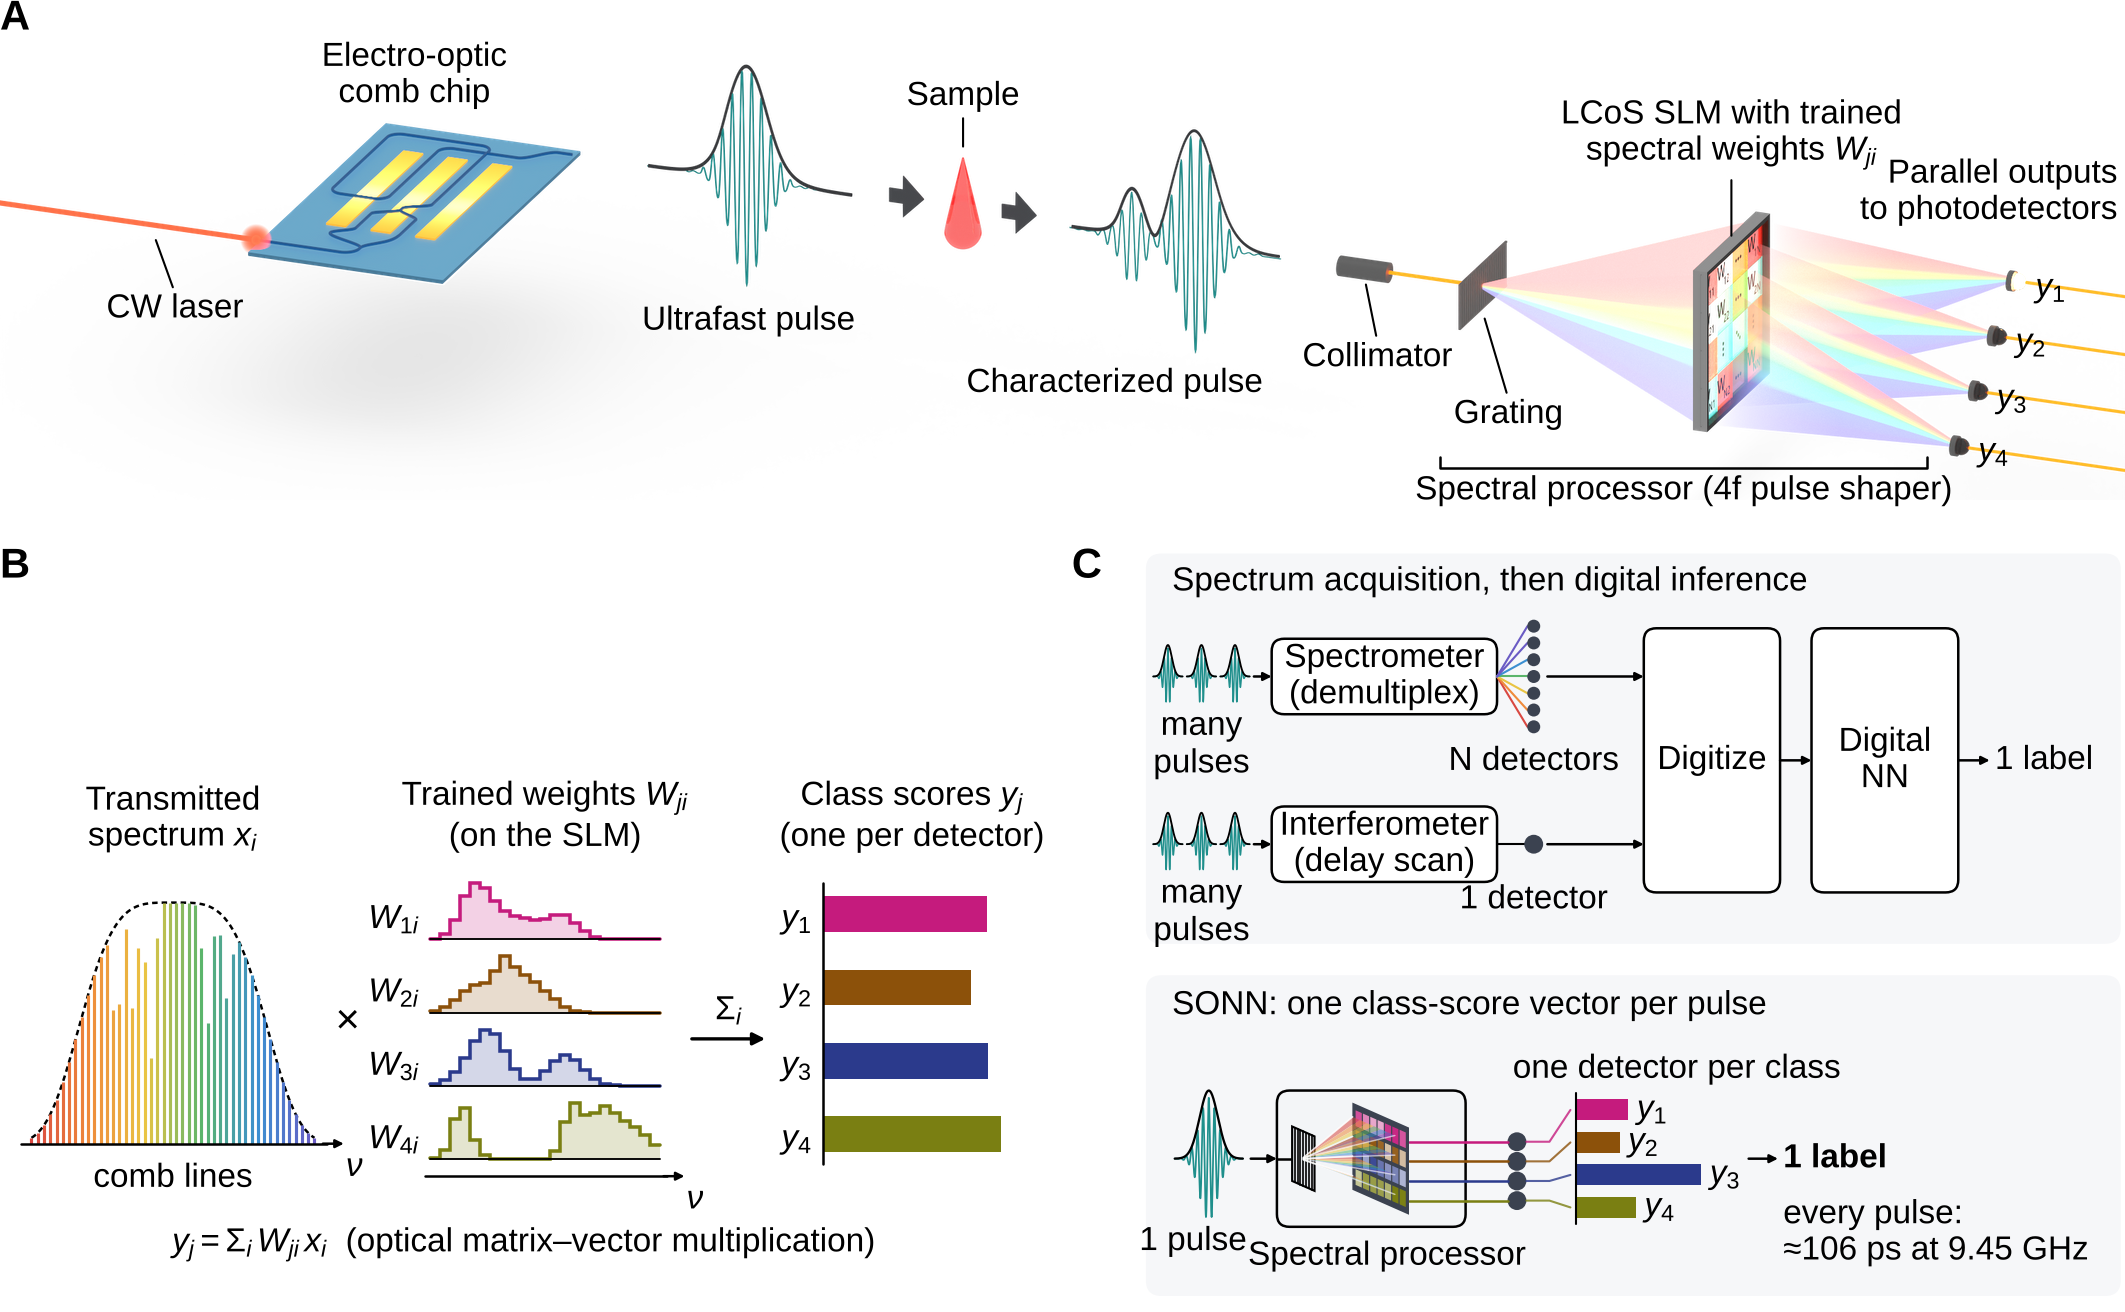
\includegraphics[width=\linewidth]{fig1.png}
  \caption{\textbf{Single-pulse spectroscopic sensing and optical computation.} (A) Three-dimensional concept of an ultrafast pulse from a chip-based electro-optic comb driven by a continuous-wave (CW) laser probing a sample (characterized pulse), undergoing learned spectral weighting on a liquid-crystal-on-silicon spatial light modulator (SLM) in a 4f pulse shaper, and producing parallel detector outputs $y_1$--$y_4$. Relay optics, the reflective modulator geometry, and fiber coupling are simplified. (B) Spectral projection. The sample-transmitted comb lines $x_i$ are weighted by trained profiles $W_{ji}$ programmed on the SLM (one weight value per spectral channel, drawn as steps), and output $j$ collects $y_j = \sum_i W_{ji}x_i$, implementing an optical matrix--vector multiplication; profiles and scores are schematic. (C) Measurement events. Spectrum-retrieval approaches first acquire the spectrum, either by demultiplexing it onto a detector array (spectrometer) or by recording an interferogram over a delay scan with a single detector, and then digitize and reconstruct it before digital inference. In the SONN architecture, a single transmitted pulse yields the complete class-score vector, with one detector per class; pulses from the 9.45-GHz comb arrive at approximately 106-ps intervals.}
  \label{fig:concept}
\end{figure}

\subsection{Single-pulse gas classification at gigahertz rates}
We demonstrated single-pulse gas classification using three room-temperature cells containing acetylene at 15~Torr, acetylene at 50~Torr, and nitrogen at 740~Torr (Fig.~\ref{fig:gas}A). These conditions present distinct transmission signatures, including two pressure levels of the same molecular species. A digital classifier was trained on absorption spectra generated using HITRAN data~\cite{gordon2022}. The learned spectral weights were then programmed onto the optical processor and held fixed throughout inference.

Three electro-optic switches, driven by an arbitrary-waveform generator synchronized to an oscilloscope, selected one gas-cell path in each pulse period. Successive pulses could therefore interrogate different cells and deliver a sequence of physical transmission spectra to the classifier. The programmed routing sequence supplied the reference labels for evaluating the optical predictions. This arrangement combined controlled changes in the spectral input with a fixed optical recognition function, enabling direct evaluation of classification across the incoming pulse stream.

At a repetition rate of 9.45~GHz, SONN produced class scores for each gated pulse position at approximately 106-ps intervals. Each prediction used the detector outputs at one gated pulse position (Materials and Methods). The pulse-resolved measurement establishes a one-to-one correspondence between sample interrogation and optical classification (Fig.~\ref{fig:gas}B). Each event is classified from the spectral information acquired during that interrogation, preserving the pulse-by-pulse sequence of the optical input.

The optical classifier achieved 77.39\% accuracy across the three gas-cell conditions, compared with 84.22\% for the digital model. This result demonstrates learned spectral discrimination resolved at the 106-ps pulse period of the 9.45-GHz comb. The 6.83-percentage-point difference quantifies the transfer from digital training to the implemented optical measurement. Together, the recognition accuracy and pulse-resolved outputs show that the programmed spectral transformation distinguishes individual pulse positions at the full comb repetition rate.

The gas task combines discrimination between molecular conditions with recognition of pressure-dependent transmission within acetylene. SONN performs this analysis through a small number of detector outputs, while processing the spectral features in parallel in the optical domain. A class-score vector is resolved at each pulse position, allowing successive positions to represent different selected cells. This controlled sequence demonstrates recognition of spectral inputs that change from one pulse to the next, the temporal resolution needed for spectroscopic classification of rapidly evolving signals.

\subsection{Direct sensing of flowing liquid mixtures}
We extended direct optical recognition to flowing liquids by coupling SONN to a microfluidic sampling system. Two computer-controlled syringe pumps delivered acetone and ethylenediamine to a mixer and sampling chip (Fig.~\ref{fig:gas}C). The acetone flow remained constant while the ethylenediamine flow changed in 200-ms steps. Pulses from the 100-MHz femtosecond comb transmitted through the mixture entered the trained spectral processor directly. This arrangement allowed the optical outputs to follow composition changes in a continuously supplied sample.

Training used 20 spectra at each integer concentration percentage, grouped into acetone ranges of 86--90\% and 91--94\%. The digital classifier achieved 93.9\% accuracy. In the dynamic experiment, the programmed flows produced nominal acetone fractions of 86\% and 92\%, and the difference between two detector outputs tracked the changes (Fig.~\ref{fig:gas}D). Assigning each 200-Hz readout sample to the state indicated by the sign of the differential output reproduced the programmed state for 95.0\% of samples (152 of 160); all eight errors fell within 15~ms of a pump transition. The detector signals were sampled at 1~MHz and averaged to a 200-Hz readout for this fluidic measurement. The liquid experiment demonstrates that the same learned spectral-projection approach can translate changes in a flowing sample directly into discriminating optical outputs.

\begin{figure}[!tbp]
  \centering
  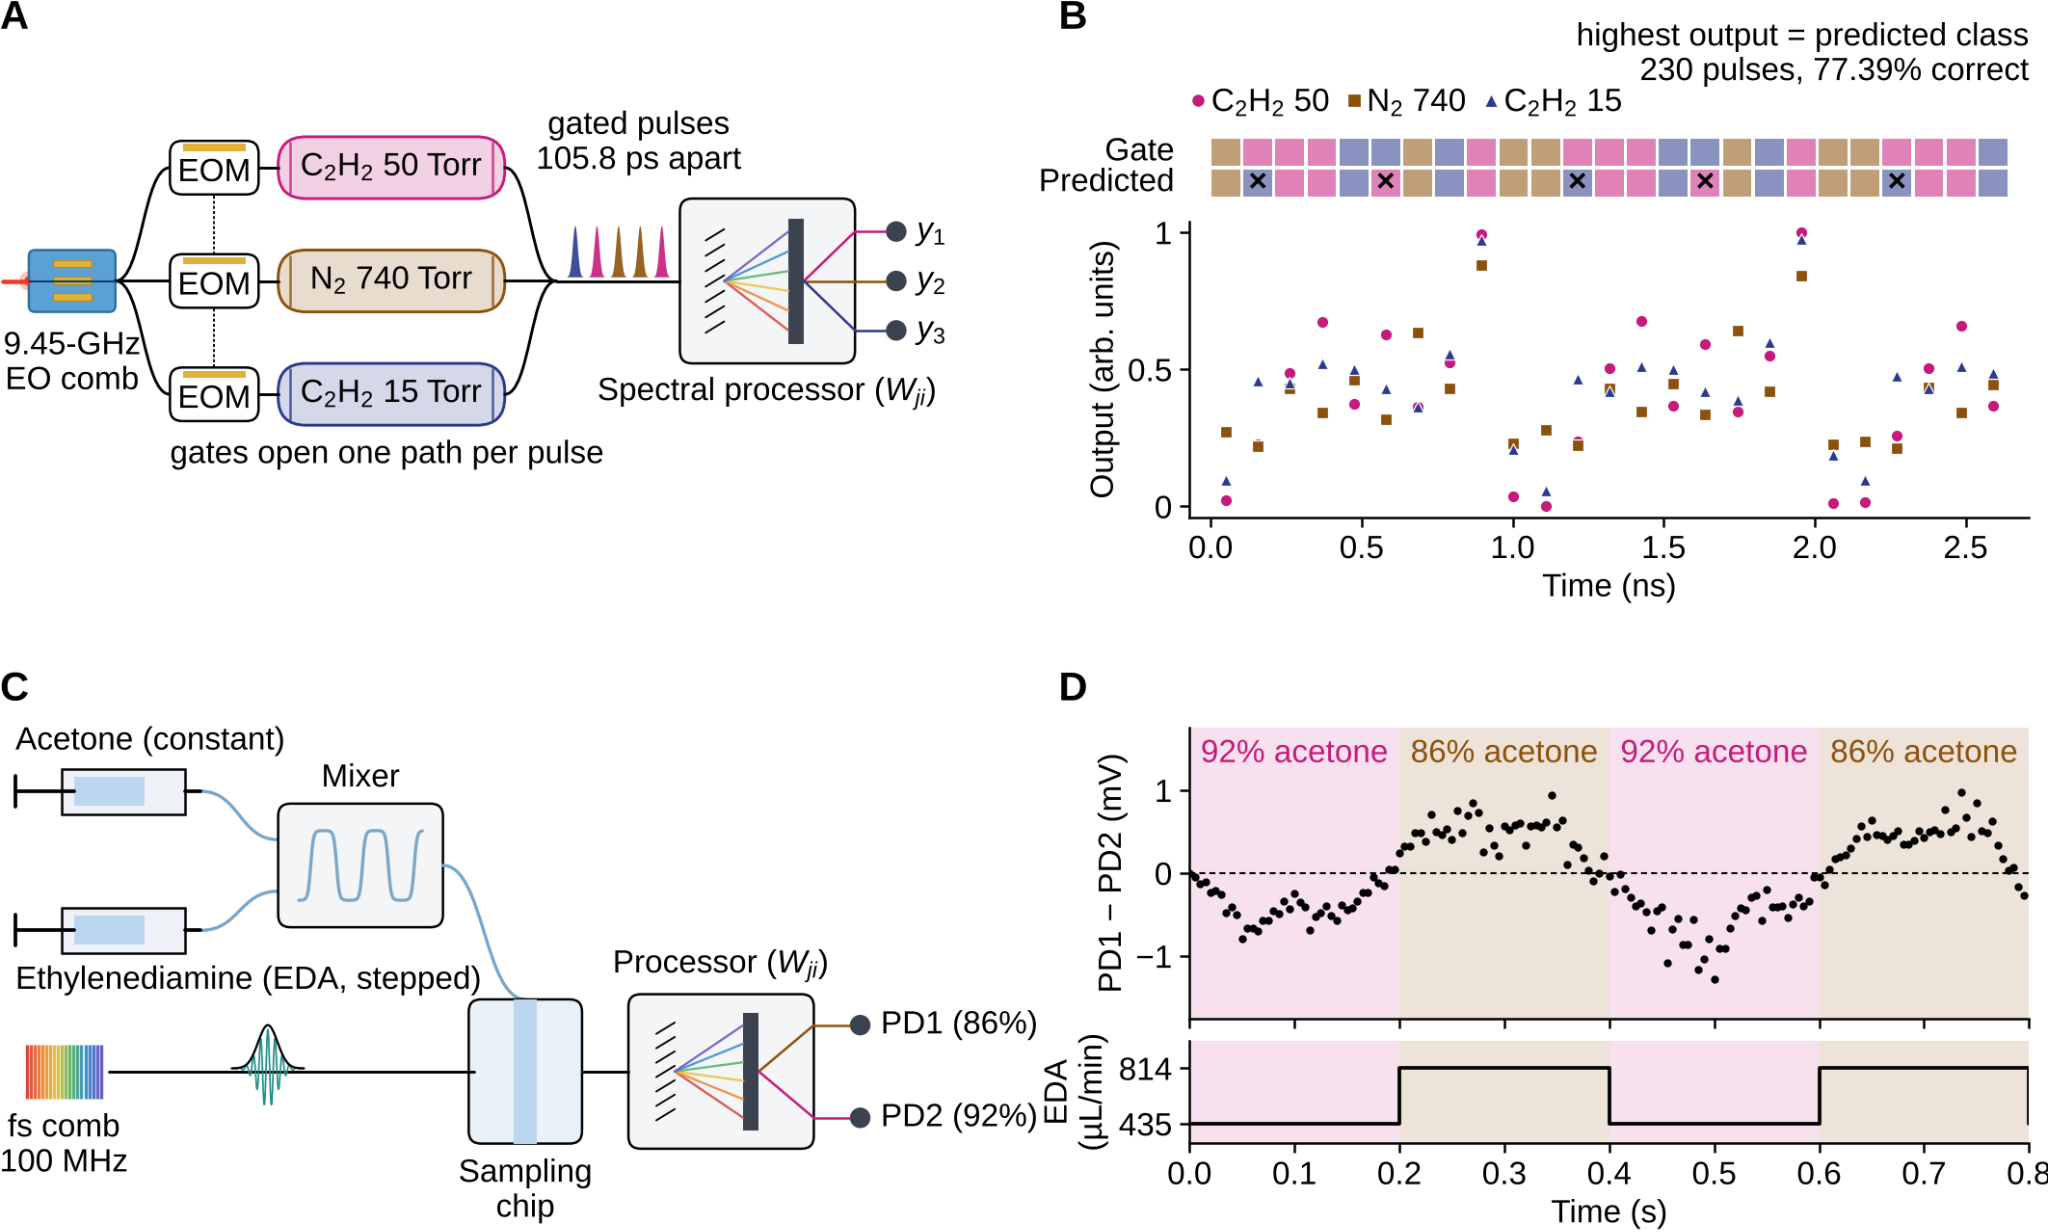
\includegraphics[width=\linewidth]{fig2.png}
  \caption{\textbf{Gas classification at 9.45~GHz and direct sensing of liquid mixtures.} (A) Synchronized electro-optic switches select one gas-cell path per pulse from a 9.45-GHz chip-based comb; the gated pulses enter the spectral processor, drawn as the grating and two-dimensional SLM of Fig.~\ref{fig:concept}A with one weight row per output. The cells contain acetylene at 15~Torr, acetylene at 50~Torr, and nitrogen at 740~Torr. (B) Calibrated detector outputs, scaled to 0--1 with the predicted class highest, for 25 consecutive gated pulses, with the programmed gate sequence and the predicted class above ($\times$ marks errors). Accuracies are evaluated over 230 pulses. Each gated pulse position yields one class-score vector, with approximately 106~ps between positions. Digital and optical accuracies are 84.22\% and 77.39\%. (C) Syringe pumps deliver acetone and ethylenediamine through a mixer and sampling chip probed by the 100-MHz femtosecond comb. The processor is drawn as in (A). (D) Differential detector output (PD1 $-$ PD2) and ethylenediamine (EDA) pump setpoint; shading marks the nominal 92\% and 86\% acetone states. Signals were sampled at 1~MHz and averaged to 200~Hz; pump settings changed in 200-ms steps. The sign of PD1 $-$ PD2 identifies the pumped state for 95.0\% of the 160 samples.}
  \label{fig:gas}
\end{figure}

\subsection{Programmable optical recognition across input types}
We evaluated the versatility of the programmed optical transformations using digit images (Fig.~\ref{fig:encoded}) and recorded Raman spectra (Fig.~\ref{fig:raman}) encoded onto the source spectrum. An input shaper prepared each spectral representation, and a second shaper applied the trained classifier weights. For handwritten digits 0--3, $28 \times 28$ MNIST images were flattened into 784-element vectors~\cite{lecun1998} and classified through four parallel outputs (Fig.~\ref{fig:encoded}, A to D). Optical accuracy reached 94.6\%, compared with 97.5\% for the digital model, demonstrating effective transfer of the trained transformation to the optical processor. Optical-spectrum-analyzer measurements confirmed that the input shaper reproduced the target profiles, with a residual spread $\sigma$ of 1.9\% for a digit image and 0.9--1.5\% for four Raman spectra (Fig.~\ref{fig:encoded}D and Fig.~\ref{fig:raman}E).

\begin{figure}[!tbp]
  \centering
  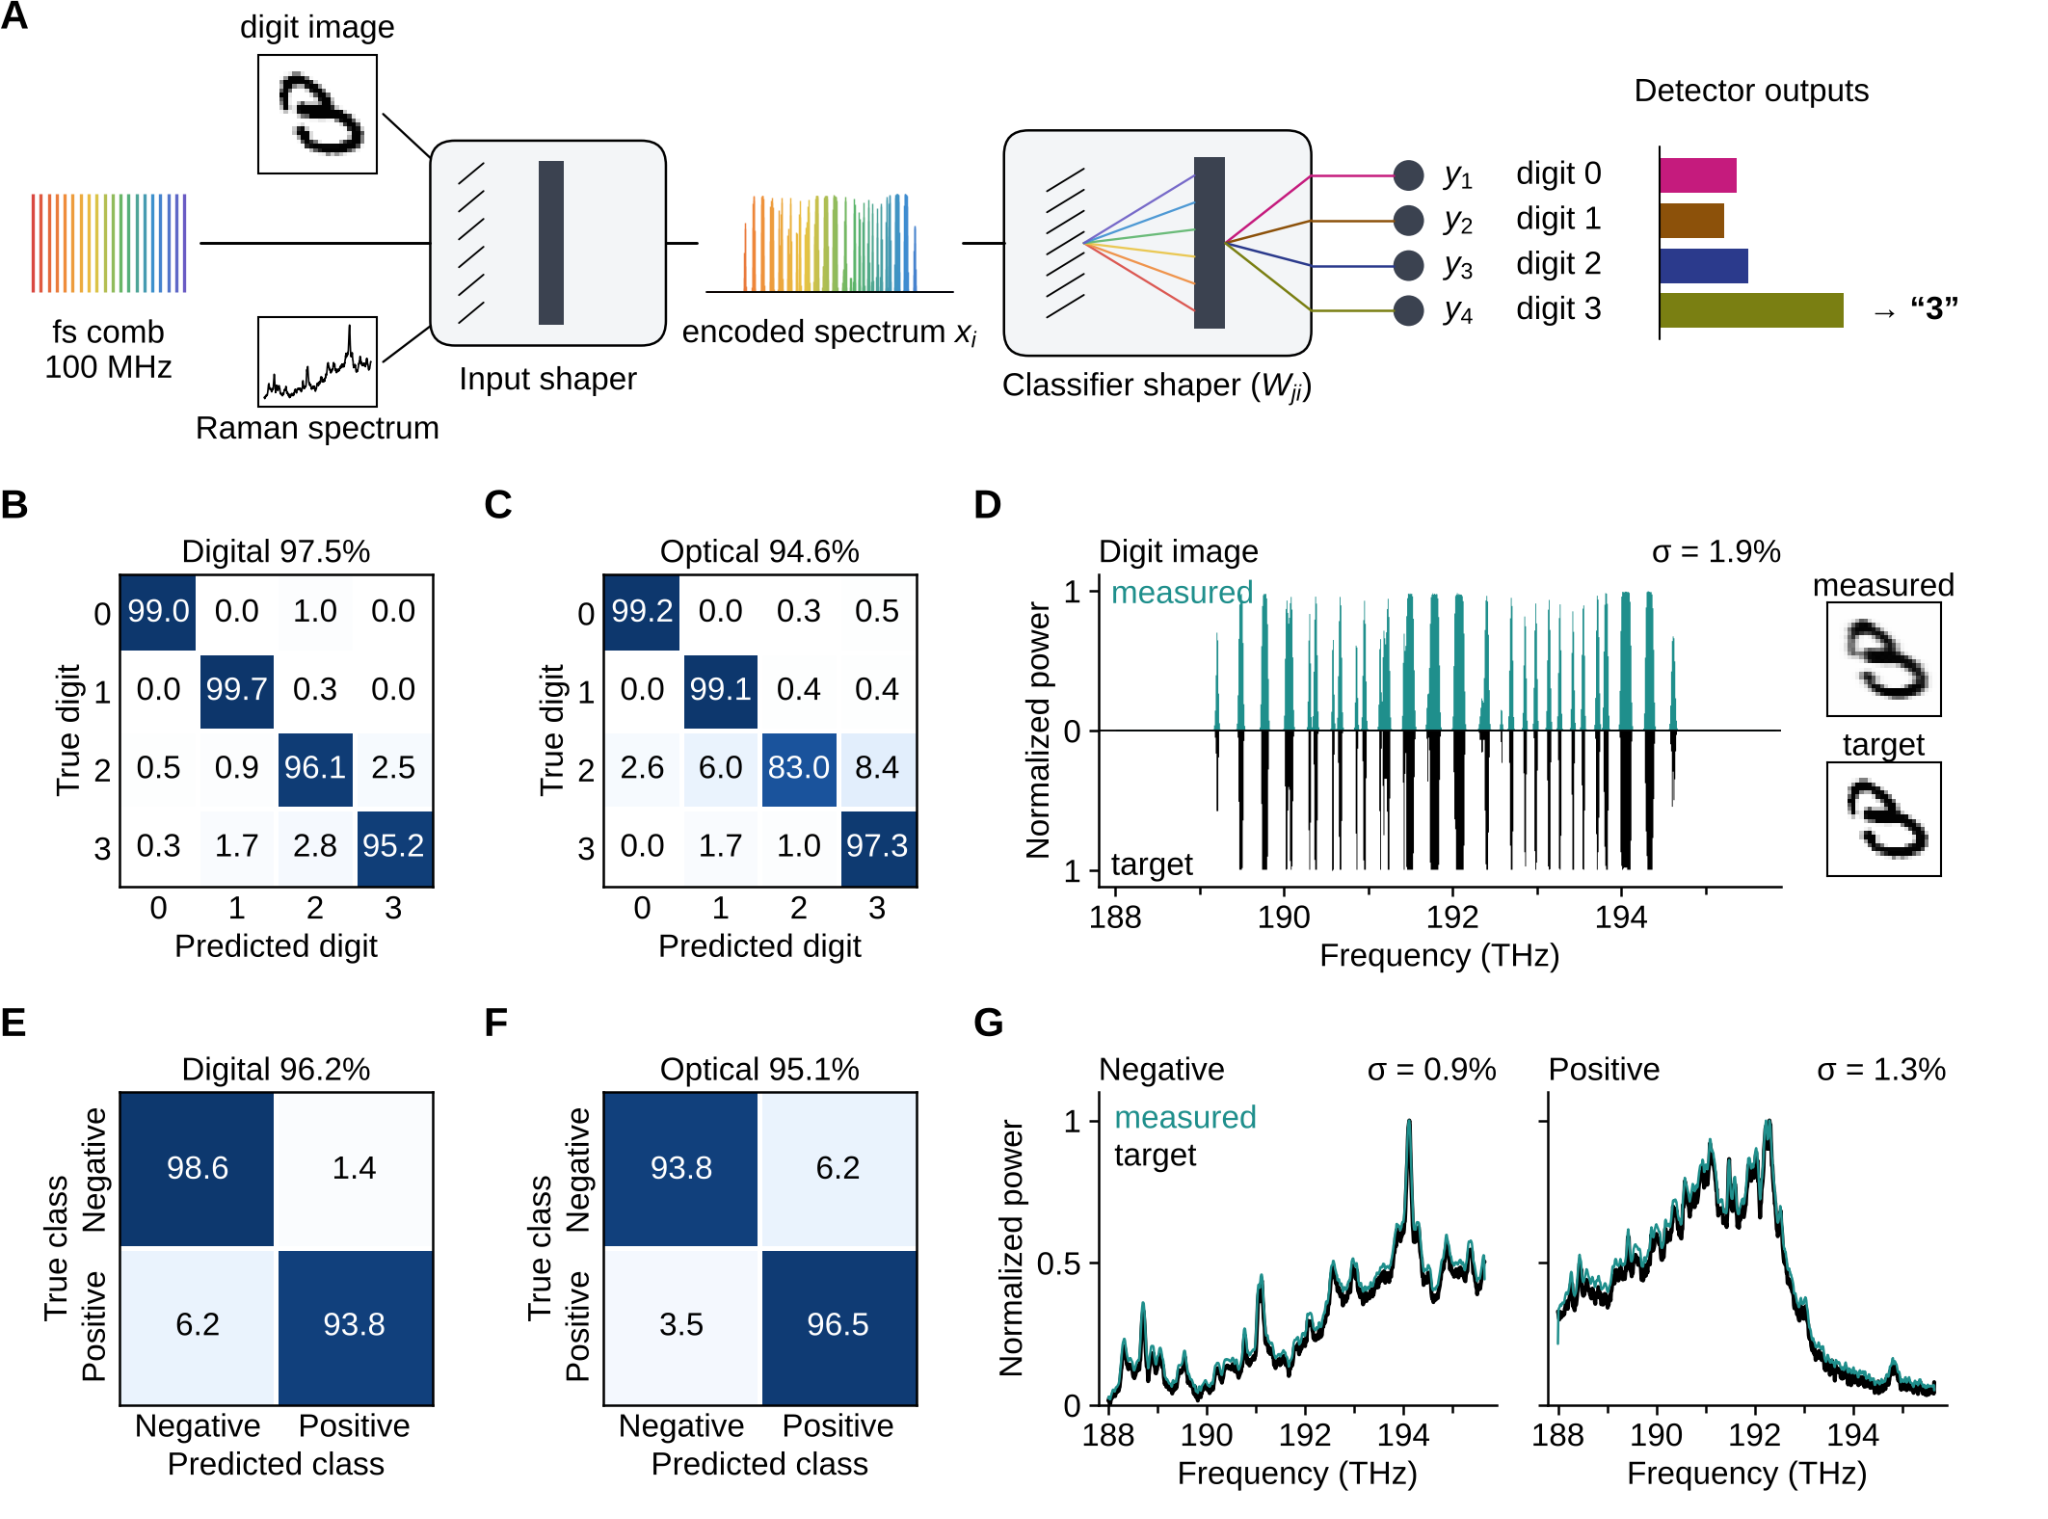
\includegraphics[width=\linewidth]{fig3.png}
  \caption{\textbf{Programmable optical classification of encoded digit images.} (A) An input spectral shaper encodes vectorized $28 \times 28$ images onto the pulses of the 100-MHz comb, and the classifier shaper applies learned weights for four outputs corresponding to digits 0--3. Each detector collects one weighted spectral projection. (B and C) Digital and optical confusion matrices for the digit task, with accuracies of 97.5\% and 94.6\%, respectively. Entries are percentages normalized within each true class. The input shaper sets the rate at which new images are loaded. Output bars in (A) are illustrative. (D) Input-encoding fidelity for a test image of digit 3: measured spectrum and target pixel values (mirrored) over 784 channels at 10-GHz spacing; insets show both as $28 \times 28$ images. The measured spectrum and the target are normalized to a maximum of 1, and $\sigma$ is half the 16th--84th percentile range of the residual (measured minus target), in percent of full scale. (E) Application concept, not measured: with spectrally dispersed illumination, each wavelength of a LiDAR pulse probes one point of the scene, so the returned pulse carries the image of a road sign on its spectrum; a multi-layer spectral processor (three SLMs in cascade, one output row per class) could then label the sign from a single pulse.}
  \label{fig:encoded}
\end{figure}

We further programmed SONN to classify surface-enhanced Raman spectra of human serum recorded with a functionalized nanofinger platform that captures B-type natriuretic peptide, a biomarker of heart attacks~\cite{zhang2025nanofinger,liu2023}. In the intended configuration (Fig.~\ref{fig:raman}A), the Raman-scattered light from the nanofinger chip enters the spectral processor directly, and the two detector outputs indicate whether the serum came from a healthy individual or from a patient before the onset of a heart attack. Because the serum samples were not available to us, the present experiment encoded the recorded spectra onto the comb with the input shaper (Fig.~\ref{fig:encoded}A) and evaluated the trained two-output classifier on 288 spectra (144 healthy, 144 patient), each from a single optical measurement of the two detector outputs (Fig.~\ref{fig:raman}B). The optical classifier identified 96.5\% of the patient spectra and 93.8\% of the healthy spectra; the corresponding digital rates were 93.8\% and 98.6\% (Fig.~\ref{fig:raman}, C and D). These results demonstrate optical discrimination of biomarker-related spectral signatures. On this balanced set, the rates correspond to overall accuracies of 95.1\% (optical) and 96.2\% (digital), and the agreement between the optical and digital results shows that the two trained weight profiles were implemented faithfully by the processor. Together with digit recognition, they establish that the spectral processor can implement different trained recognition functions by updating its weight profiles. The two encoded-input experiments broaden the demonstrated applications of the hardware beyond direct transmission sensing.

\begin{figure}[!tbp]
  \centering
  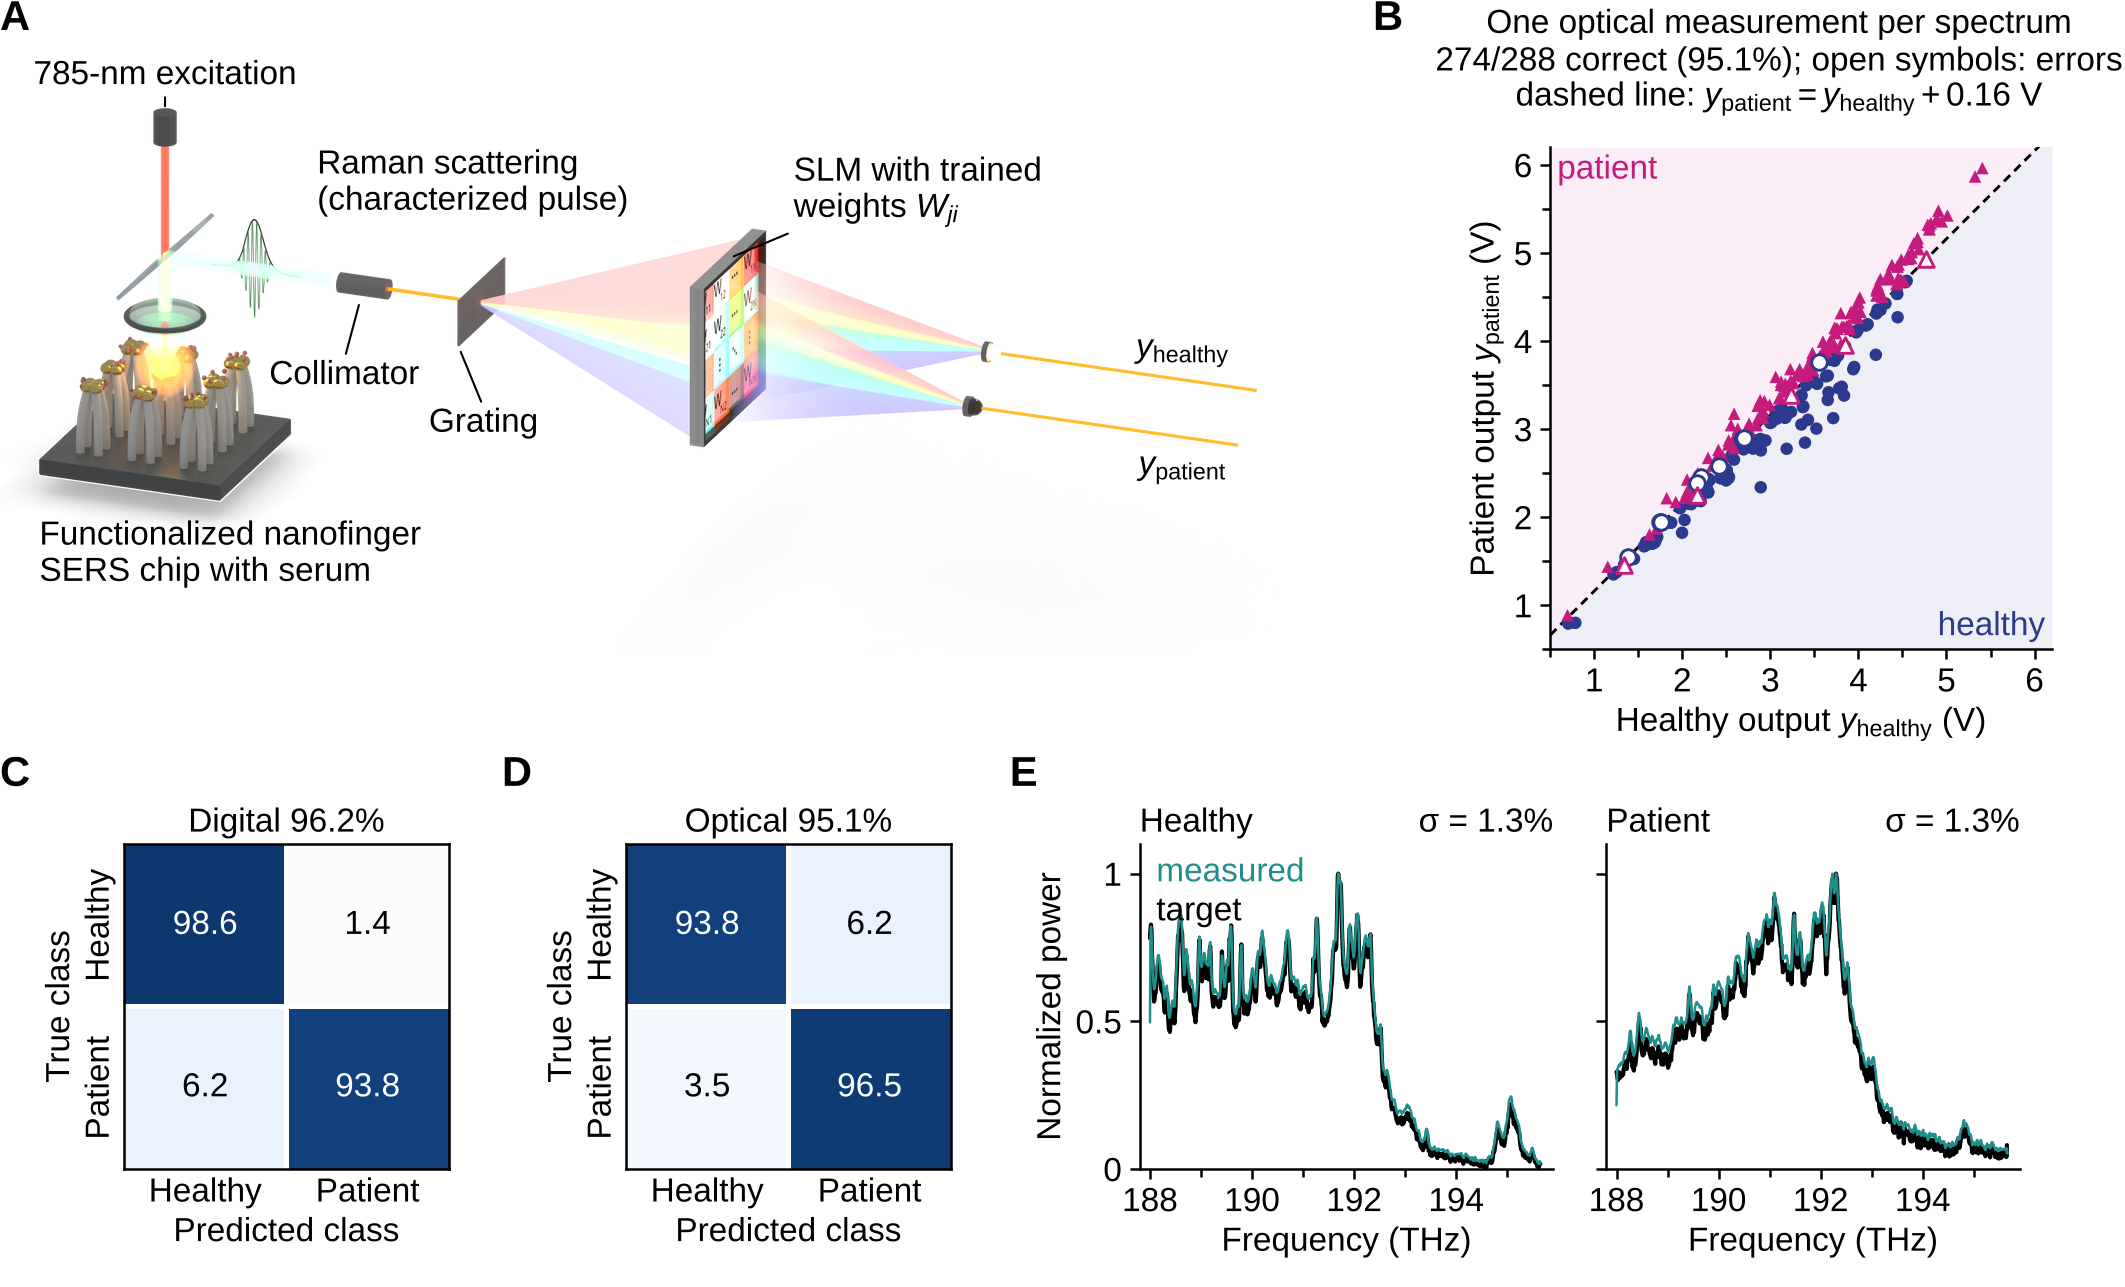
\includegraphics[width=\linewidth]{fig4.png}
  \caption{\textbf{Early warning of heart attacks from serum Raman spectra.} (A) Intended direct-coupled configuration (concept), drawn with the processor of Fig.~\ref{fig:concept}A: serum on a functionalized nanofinger SERS chip is excited at 785~nm, and the Raman-scattered light (green pulse) is collected and passes directly through the grating and SLM, whose two trained weight rows yield one output for healthy and one for patient serum. In the present experiment the serum samples were not available, so Raman spectra recorded with this platform~\cite{zhang2025nanofinger,liu2023} were encoded onto the comb by the input shaper (Fig.~\ref{fig:encoded}A) before the classifier. (B) The two detector outputs for each of the 288 evaluated spectra (144 healthy, 144 patient), one optical measurement per spectrum. The dashed line is the decision boundary $y_{\mathrm{patient}} = y_{\mathrm{healthy}} + 0.16$~V; open symbols mark the 14 misclassified spectra. (C and D) Digital and optical confusion matrices for the same spectra, normalized within each true class; overall accuracies are 96.2\% and 95.1\%. (E) Input-encoding fidelity for one healthy and one patient spectrum over 766 channels at 10-GHz spacing: measured spectrum and target, each normalized to a maximum of 1; $\sigma$ is half the 16th--84th percentile range of the residual (measured minus target), in percent of full scale. The four encoded Raman spectra measured gave $\sigma = 0.9$--$1.5$\%.}
  \label{fig:raman}
\end{figure}


\FloatBarrier
\section{Discussion}
SONN establishes single-pulse spectroscopic classification at a 9.45-GHz event rate by combining sample interrogation, learned spectral weighting, and parallel readout within a single optical measurement. In this architecture, each transmitted pulse supplies the complete class-score vector, linking recognition directly to the physical interrogation. The advance lies in this temporal capability: a trained optical transformation processes successive sample-derived spectra as they arrive, with fixed weights. The gas experiment demonstrates this capability at gigahertz rates, while the liquid, digit, and Raman results establish the flexibility of the underlying spectral processor.

This demonstration advances direct spectral recognition into a gigahertz operating regime. Earlier approaches established parallel optical projections and sub-megahertz spectral pattern updates~\cite{vornehm2014,huh2018}, while spectral kernel machines reported a 2-$\mu$s bandwidth-limited inference time in the visible band~\cite{zhang2025kernel}. The photonic edge-intelligence platform identifies an approximately 100-MHz operating range for its prototype~\cite{zhang2025edge}. Recent all-optical recurrent computing reaches 100-GHz-class clocks, with waveform classification obtained by pooling a sequence of output pulses~\cite{li2026}. SONN instead derives the optical classification output at each sample-transmitted pulse position. This event-based measurement connects the demonstrated throughput to individual spectroscopic interrogations.

The comparison with scanning Michelson, dual-comb, and convolutional spectroscopy concerns the information acquired per event. Their spectrum-retrieval workflows assemble measurements over a delay scan, an interferogram, or a sequence of tuned spectral responses~\cite{yang2021,picque2019,coddington2016,long2024,yao2026}. The SONN architecture obtains the trained projections concurrently from one sample-transmitted pulse, removing the need to assemble such a sequence for each classification. The resulting measurement is task-specific: spectral details not retained in the output scores are unavailable for later analysis, and a new recognition task may require reprogramming the weights. Full spectral retrieval remains valuable when the relevant signatures are not known in advance.

The ability to classify each interrogation creates opportunities for studying signals whose distinguishing features evolve between successive measurements. Learned spectral projections can select signatures of interest during acquisition and retain their temporal sequence in a compact set of output channels. Applied to transient chemistry or evolving material states, this approach could identify spectral events that repeated-shot averaging would obscure. The controlled gas-routing experiment demonstrates pulse-resolved recognition of changing physical inputs. Extending this capability to dynamic samples and coupling the outputs to suitable feedback hardware offers a route toward spectroscopy that responds to the phenomena it measures.

The measured digital-to-optical accuracy difference provides a quantitative target for improving the high-speed system. More accurate spectral calibration, closer matching of training spectra to measured transmission, and optimized detector readout offer routes to improved fidelity; their individual contributions remain to be established. Simultaneous readout of all output channels at the full repetition rate is the next step. Optical loss, the photon budget per pulse, and the allocation of light among outputs will guide scaling to larger class sets. Spatial information can enter the same pipeline: with spectrally dispersed illumination, each wavelength probes one point of a scene and the returned pulse carries the image on its spectrum, so a multi-layer spectral processor could label objects such as road signs pulse by pulse (Fig.~\ref{fig:encoded}E). These considerations define concrete directions for advancing the platform while retaining its central operating principle. By producing learned spectral features at the timescale of individual probing pulses, SONN unites ultrafast spectroscopy and optical computation for real-time recognition at gigahertz rates.

% ---------- Back matter ----------
\section*{Acknowledgments}
\textbf{Acknowledgments:} \todo{Add individuals and facilities to acknowledge.}

\textbf{Funding:} \todo{Add funding sources and grant identifiers.}

\textbf{Author contributions:} \todo{Assign the contributions agreed by all authors.}

\textbf{Competing interests:} \todo{Provide the authors' declaration, including relevant patents or commercial interests where applicable.}

\textbf{Data and materials availability:} \todo{Provide repository links or accession identifiers for source data, training code, trained weights, calibration files, and analysis scripts. Explain access conditions for reused Raman data.}

% ---------- References ----------
\bibliographystyle{unsrtnat}
\bibliography{refs}

% ---------- Supplementary Materials ----------
\section*{Supplementary Materials}
Materials and Methods (separate file, \texttt{supplement.tex})

\end{document}
